\chapter{Main Concepts}

% Describe your own work (how you reached your goal) and take care to motivate your choices. Don't just describe all the things you did – tell us why.
% Background theory and main concepts

\section{Labeled Ordered Rooted Tree}

Ordered labeled trees are trees in which hte left-to-right orer among siblings is significant \cite{shasha1990a}.

An HTML document is a hierarchical tree structure with a defined order, i.e. depth-first pre-order traversal. It has a single root node (<HTML> element) and contains nodes from a finite set of elements: <P>, <DIV>, <H1>, <STRONG>, etc. Each element type has semantic associated with it.

% TODO rewrite from [PARAMESWARAN'11]
[TODO] Ordered Labeled Trees : Let w be a webpage. We represent w as an ordered, labeled tree corresponding to the parsed HTML DOM tree of the webpage. As an example, consider Figure 1, represent- ing the HTML of an IMDB page. The children of every node areordered, (e.g., in Figure 1, the node corresponding to head is or- dered before the node corresponding to body among the children of the root) and every node has a label from a set of labels L (e.g., the root has a label html ). The label of a node essentially indicates the type of the node.

In addition, the nodes at the leaves are text nodes (depicted in Figure 1 as text in gray). For instance, the first leaf has textual content “ Title ”. Since we are primarily interested in structural changes, for our algorithms we replace all HTML text nodes with nodes having special label “ TEXT ”. (In Appendix B.4.1, we de- scribe some extensions that we use to leverage the textual content information in addition to structure.)

We define two webpages w 1 and w 2 to be isomorphic, written as w 1 = w 2 , if they have identical structure and labels, i.e. there is a bijection b between the nodes in w 1 and w 2 that respects labels and order. Two nodes n 1 in w 1 and n 2 in w 2 are said to be isomorphic (n 1 = n 2 ), if w 1 = w 2 and n 1 and n 2 are mapped to each other under the bijection.

We assume that each webpage w has a distinguished node d(w) containing the textual information of interest, e.g., the node con- taining the number of votes on an imdb.com movie page. For ease of presentation, we assume that there is a single distinguished node in each page. Appendix C describes how our techniques can be used to handle multiple distinguished nodes, e.g., extracting the list of actors in a movie page

---

pre-order, depth-first traversal of DOM nodes involved [see 
http://www.w3.org/TR/html5/infrastructure.html\#terminology
http://www.w3.org/TR/dom/\#element


\section{XML}

[TODO] W3Org notations: DOM, XML, XPath, XSLT ,etc. ref \cite{Myllymaki02robustweb}.

% http://en.wikipedia.org/wiki/XML
Extensible Markup Language (XML) is a markup language that defines a set of rules for encoding documents in a format which is both human-readable and machine-readable. It is defined by the W3C's XML 1.0 Specification[2] and by several other related specifications,[3] all of which are free open standards.[4]

% http://en.wikipedia.org/wiki/Document_Object_Model
The Document Object Model (DOM) is a cross-platform and language-independent convention for representing and interacting with objects in HTML, XHTML, and XML documents.[1] The nodes of every document are organized in a tree structure, called the DOM tree. Objects in the DOM tree may be addressed and manipulated by using methods on the objects. The public interface of a DOM is specified in its application programming interface (API).

% http://en.wikipedia.org/wiki/XML
XPath defines a syntax named XPath expressions which identifies one or more of the internal components (elements, attributes, and so on) included in an XML document. XPath is widely used in other core-XML specifications and in programming libraries for accessing XML-encoded data.

% http://en.wikipedia.org/wiki/XML
XSLT is a language with an XML-based syntax that is used to transform XML documents into other XML documents, HTML, or other, unstructured formats such as plain text or RTF. XSLT is very tightly coupled with XPath, which it uses to address components of the input XML document, mainly elements and attributes.


\section{Data Records}

% TODO [ZHAI'05]
[TODO] The MDR algorithm is based on two observations about data
records in a Web page and an edit distance string matching
algorithm [2] to find data records. The two observations are:

\begin{figure}[h]
	\centering
	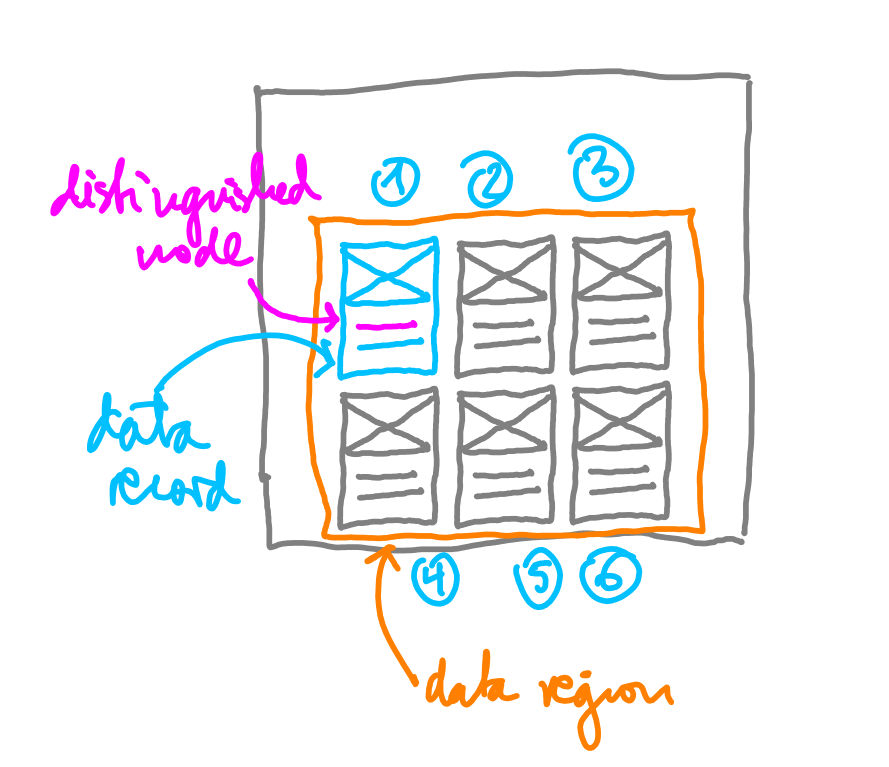
\includegraphics[width=0.5\linewidth]{figures/method}
	\caption{Inputs / outputs of the wrapper}
	\label{fig:method}
\end{figure}

1. A group of data records that contains descriptions of a set of
similar objects are typically presented in a contiguous region
of a page and are formatted using similar HTML tags. Such a
region is called a data record region (or data region in short).
For example, in Figure 1(A) two books are presented in one
contiguous region. They are also formatted using almost the
same sequence of HTML tags. If we regard the HTML tags of
a page as a long string, we can use string matching (e.g., edit
distance [2]) to compare different sub-strings to find those
similar ones, which may represent similar data records.
The problem with this approach is that the computation is
prohibitive because a data record can start from any tag and
end at any tag. A set of data records typically does not have
the same length in terms of its tag strings because it may not
contain exactly the same pieces of information (see Figure
1(A)). The next observation helps to deal with this problem.

2. The nested structure of HTML tags in a Web page naturally
forms a tag tree. For example, Figure 2 shows an example tag
tree. In this tree, each data record is wrapped in 3 TR nodes
with their sub-trees under the same parent TBODY. The two
data records are in the two dash-lined boxes. Our second
observation is that a set of similar data records are formed by
some child sub-trees of the same parent node.

It is unlikely that a data record starts in the middle of a child
sub-tree and ends in the middle of another child sub-tree.
Instead, it starts from the beginning of a child sub-tree and
ends at the end of the same or a later child sub-tree. For
example, it is unlikely that a data record starts from TD* and
ends at TD (Figure 2). This observation makes it possible to
design a very efficient algorithm based on edit distance string
comparison to identify data records because it limits the tags
from which a data record may start and end in a tag tree. 1

Experiments show that these observations work very well. By no
means do we assume that a Web page has only one data region
that contains data records. In fact, a Web page may contain a few
data regions. Different regions may have different data records.

\section{Edit Tree Distance}

% TODO rewrite [Zhai'05]

[TODO] Similar to string edit distance, tree edit distance [31, 30] between
two trees A and B (we are only interested in labeled ordered
rooted trees) is the cost associated with the minimum set of
operations needed to transform A into B. In the classic
formulation, the set of operations used to define tree edit distance
includes three operations: node removal, node insertion, and node
replacement. A cost is usually assigned to each of the operations.
Solving the tree edit distance problem is often assisted by finding
a minimum-cost mapping between two trees [30]. The concept of
mapping [30] is formally defined as:

Let X be a tree and let X[i] be the ith node of tree X in a preorder
walk of the tree. A mapping M between a tree A of size n 1 and a
tree B of size n 2 is a set of ordered pairs (i, j), one from each tree,
satisfying the following conditions for all (i 1 , j 1 ), (i 2 , j 2 ) in M:

(1) i 1 = i 2 iff j 1 = j 2 ;
(2) A[i 1 ] is on the left of A[i 2 ] iff B[j 1 ] is on the left B[j 2 ];
(3) A[i 1 ] is an ancestor of A[i 2 ] iff B[j 1 ] is an ancestor of B[j 2 ].

Intuitively, the definition requires that each node can appear no
more than once in a mapping and the order between sibling nodes
and the hierarchical relation between nodes are both preserved.
Figure 8 shows a mapping example.

Several algorithms have been proposed to address the problem of
finding the minimum set of operations (i.e., the one with the
minimum cost) to transform one tree into another. All the
formulations have complexities above quadratic [10]. It has also
been shown that if the trees are not ordered, the problem is NP-
complete [36]. In [30], a solution based on dynamic programming
is presented. The algorithm has a complexity of O(n 1 n 2 h 1 h 2 ),
where n 1 and n 2 are the sizes of the trees and h 1 and h 2 are heights
of the trees. In [32][10], two other algorithms are also presented
with similar complexities.

% TODO [PARAMESWARAN'11]

[TODO] Edit Operations : We are interested in modeling the scenario when
the webpages undergo structural changes. Each change is one of
three edit operations: insertion of a node (i.e., insert a node x as a
child of another node y, and assign some subsequence of y’s chil-
dren as x’s children,) deletion of a node (i.e., delete node x and
assign all of x’s children as its parent’s,) and substitution of the
label of a node.

Each edit operation takes an ordered labeled tree and creates a
new ordered labeled tree, i.e., the labels and structure of the new
tree are the same as in the old tree, except for the single node that
was edited (either inserted, deleted, or substituted). Thus, apart
from one node that may have been inserted or deleted, there is an
implicit mapping between the old and new versions of the nodes
in the two trees. Furthermore, these mappings can be “composed”
across various edits, effectively providing a mapping between the
first and last trees for a sequence of edit operations. Note that the
only nodes in the first tree that do not have a mapping are those
that are deleted at some point in the sequence of edits, and the only
nodes in the last tree that do not have a mapping are those that were
inserted at some point in the sequence of edits.

A sequence s of edit operations is defined to be an edit script.
We let s(w) denote the new version of the webpage obtained by
applying the operators in s in sequence to w. We use s(n), n in w,
to denote the node in s(w) that n maps to when edit script s is
applied. (Note that we are overloading function s, however the use
should be clear from the context.)

Evolution of Webpages : We assume there is some evolution pro-
cess pi that takes a webpage w and creates a new version of the
webpage pi(w) by performing a sequence of edit operations on w
that include insertion of nodes, deletion of nodes and substitution of
labels. Thus pi is essentially an edit script. Since we are primarily
interested in structural changes, we ignore any changes that are not
to the ordered labeled tree. However, we are not given what pi is;
we are only provided the new version of the webpage w = pi(w).

% TODO more sources

\cite{de2004a}

\section{Wrapper}

The term originates from information system integration domain \cite{Chang:2006:SWI:1159162.1159300}, where a proxy interface abstracts away the complexity of accessing a data source. 

% TODO [PARAMESWARAN'11]

[TODO] Page-level Wrapper Robustness : The problem is formally de-
fined in Section 2, and is the focus of this paper. We are given a
page w along with the locations of the labeled nodes, and we want
to extract the information from a future version of w. We consider
a change model that captures how webpages evolve over time by
looking at the likelihood of all possible changes. Change models
for webpages have been previously proposed [17], along with algo-
rithms for learning models based on archival data. Given a model,
we give algorithms to construct a wrapper that gives the most likely
locations of the labels in the new version. We consider two differ-
ent notions of robustness : probabilistic robustness, that looks at
wrappers that are most likely to work in the future in expectation,
and adversarial robustness, that looks at wrappers that are most
likely to work in the future in the worst-case.

Wrappers and Robustness : Let w be a webpage with a distin-
guished node d(w). We want to construct a wrapper that extracts
from future versions of w. Let w = pi(w) be a new version of the
webpage. We want to find the location of distinguished node in w .
We assume that the distinguished nodes are never deleted when
webpages evolve. For instance, an IMDB movie webpage will al-
ways contain the number of votes even though the webpage may
change. It is reasonable to assume this since the content of interest
is usually an important part of the webpage, and we only intend to
be robust to cosmetic changes and other peripheral changes (e.g.,
changes to ads) that do not affect the main content. Thus, there
is a single distinguished node d(w ) = pi(d(w)) in the new tree
w = pi(w), namely the node that the distinguished node d(w) is
mapped to on applying edits pi.

As an example, consider Figure 3. Every node in the ordered
labeled trees in this figure has the label “a”. The second leaf in T 1 is
the distinguished node (with a dashed box around it). Consider tree
T 1 and T 2 . Let us say tree T 2 is obtained from T 1 by an edit script
pi that deletes the first leaf in T 1 . Then, the distinguished node in
T 2 is now the first leaf (displayed using a dashed box in T 2 .) On
the other hand, tree T 3 is obtained from T 1 by an edit script pi that
deletes one of the last 3 leaves of T 1 . The distinguished node in T 3
is now the second node. Note that T 2 and T 3 are isomorphic trees.
We are now ready to define what we mean by a wrapper.
A wrapper is a function fi from a webpage to a node in the
webpage. We say that a wrapper fi works on a future version
w of a webpage w, denoted fi |= w , if fi(w ) = d(w ).

If fi(w ) = d(w ), then we say that the wrapper has failed or has
broken. As an example, consider the wrapper “extract the second
leaf” for Figure 3. If we apply this wrapper to T 2 , it fails. On the
other hand, if we apply it to T 3 , it works.

Our objective is to construct page-level wrappers which are im-
mune to pi, i.e., wrappers which continue to extract the distinguished
node in the new versions of webpages. We consider two different
models for the evolution process pi.

% vim:wrap linebreak nolist:
